%% Template for EU deliverable, using the deliverable.sty style file

\documentclass[12pt,a4paper,twoside]{article}

%% common package
\usepackage[headers]{deliverable}
\usepackage{xspace}
\usepackage{verbatim}
\usepackage[usenames]{color}
\usepackage[usenames,dvipsnames]{xcolor}
\usepackage{graphicx}
\usepackage{url}
\usepackage{array}
%%

%%insert here other packages needed by sections

%%

%%%%%%%%%%%%%%%%%%%%%%%%%%%%%%%%%%%%%%%%%%%%%%%%%%%%%%%%%%%%%%%%%%%%%%%%%%%%%%
%%% Titlepage
%%%%%%%%%%%%%%%%%%%%%%%%%%%%%%%%%%%%%%%%%%%%%%%%%%%%%%%%%%%%%%%%%%%%%%%%%%%%%%

% declaration of variables used in style
\deliverableDocnumber{D7.1}
\deliverableTitle{Dissemination and exploitation plan.}

\deliverableAuthor{Francesco Nori}
\deliverableResponsiblePartner{IIT}
\deliverableAffiliation{% Insert here authors affiliations
 $^1$ IIT
}

\deliverableReviewer{Francesco Nori}
\deliverableCoordinator{Francesco Nori}
\deliverableActivityNumber{n} %% n=1,..,10
\deliverableActivity{RTD}
\deliverableDoctype{Deliverable} %% or Prototype
\deliverableClassification{Public} % or Consortium
\deliverableDistribution{Consortium} %
\deliverableStatus{Draft} % Draft or Final
\deliverableDeliveryDate{28/2/2014}
\deliverableFile{D7.1.pdf} % please do not use "-" in the name
\deliverableVersion{1.0}
\deliverableDate{Feb.~28, 2014}
\deliverableYear{2014}
\deliverablePages{\pageref{LastPage}}
\deliverableChangelog{v.1.0 & Feb 19, 2013 & First draft %%\\\hline
%%              v.2.0 & Feb 20, 2007 & Final version
}
\deliverableProjectStartingDate{1st March 2013}
\deliverableProjectEndDate{28th February 2017}
\deliverableProjectAcronym{CoDyCo}
\deliverableProjectTitle{Whole-Body Compliant Dynamical Contacts in Cognitive Humanoids}
 \deliverableContractNumber{600716}
 \deliverableProjectCoordinator{Istituto Italiano di Tecnologia}
 \deliverableProjectUrl{www.codyco.eu}
 \deliverableFrameworkProgramme{FP7}
 
 \deliverableWorkpackage{deliv WP7}
 \deliverableEditors{Francesco Nori and Francesca Boscolo}
 \deliverableContributors{Francesco Nori and Francesca Boscolo}
 \deliverableReviewers{}
\deliverableAbstract{In this document we provide a comprehensive exploitation plan }
\deliverableReviewers{}
\deliverableKeywordList{Exploitation, results, transfer, intellectual properties, promotion.}

%%%%%%%%%%%%%%%%%%%%%%%%%%%%%%%%%%%%%%%%%%%%%%%%%%%%%%%%%%%%%%%%%%%%%%%%%%%%%%
%%% Sections
%%%%%%%%%%%%%%%%%%%%%%%%%%%%%%%%%%%%%%%%%%%%%%%%%%%%%%%%%%%%%%%%%%%%%%%%%%%%%%

%% constants
\newcommand{\botegoCaps}{BOTEGO}
\newcommand{\certhCaps}{CERTH}
\newcommand{\cybionCaps}{CYBION}
\newcommand{\nuigCaps}{NUIG}
\newcommand{\ubitechCaps}{UBITECH}

%%
%%%%%%%%%%%%%%%%%%%%%%%%%%%%%% BEGIN DOCUMENT
\begin{document}

\deliverableMaketitle

%%TODO move to style
\newcolumntype{L}[1]{>{\raggedright\let\newline\\\arraybackslash\hspace{0pt}}m{#1}}
\newcolumntype{C}[1]{>{\centering\let\newline\\\arraybackslash\hspace{0pt}}m{#1}}
\newcolumntype{R}[1]{>{\raggedleft\let\newline\\\arraybackslash\hspace{0pt}}m{#1}}

\textbf{Document Revision History}
\begin{center}
\begin{tabular}{|C{2cm}|C{3cm}|p{5cm}|C{4cm}|}
\hline
\textbf{Version}&\textbf{Date}&\textbf{Description}&\textbf{Author}\\\hline
First draft & 19 Feb 2014 & This version mainly contains the information that was collected via email from the partners. Partners provided IIT with details on their technological transfer facilities. & Francesco Nori\\\hline
\end{tabular}
\end{center}
 
 \clearpage

\newpage
\renewcommand*\contentsname{Table of Contents}
\renewcommand*\listfigurename{Index of Figures}
\tableofcontents
\newpage
% \listoffigures
\newpage

%%%%%%%%%%%%%%%%%%%%%%%% Start deliverable content here.

\section{Introduction}
This deliverable presents the dissemination and exploitation plan. With respect to the plan proposed in the CoDyCo description of work, we provide additional information mainly concerning the technological transfer facilities available for partners and the possible exploitation of the project results. More details can be found in Section ``B3. IMPACT'' of the CoDyCo description of work, with specific attention to ``B3.2 PLAN FOR THE USE AND DISSEMINATION OF FOREGROUND''. In the present deliverable no information is given about the dissemination plan and again the interested read should refer to the description of work, Section ``B3.2.1 DISSEMINATION PLAN''.

\section{Executive Summary}
The present deliverable is organized in two sections. Section \ref{sec:tt} presents partner by partner the available technological transfer resources. Section \ref{sec:exploit} gives a few more details on the possible exploitation areas. 

\section{Technological transfer facilities} \label{sec:tt}
In this section we describe the technological transfer facilities per each of the CoDyCo partners. We discuss in particular relevant information such as number of people involved in the facilities, a brief description of the activities and a tentative list of companies which collaborate with the institution. 

\subsection{The IIT technological transfer facility}

\subsubsection{Name of the office for tech transfer}
The IIT has a Technology Transfer office directed by Salvatore Majorana: salvatore.majorana@iit.it.

\subsubsection{Number of people involved in the activity }
The office has two divisions, 9 people and three more will join the group from june 2014 in licensing and industrial alliances division. Current members are:

\begin{itemize}
\item Lorenzo De Michieli, manager of licensing and industrial liaison division: lorenzo.demichieli@iit.it

\item Fulvio Puzone, business developer (licensing and industrial liaison): fulvio.puzone@iit.it

\item Marcella Impoco, IP and contracts lawyer (licensing and industrial liaison): marcella.impoco@iit.it

\item Federica Fordred, administration and finance: federica.fordred@iit.it

\item Lorenzo Rossi, manager IP protection division: lorenzo.rossi@iit.it

\item Augusta Galano, senior patent professional (IP protection): augusta.galano@iit.it

\item Roberta Sulcis, senior patent professional (IP protection): roberta.sulcis@iit.it

\item Matteo Faccenda, junior patent professional (IP protection): matteo.faccenda@iit.it
\end{itemize}

\subsubsection{Rough estimate of the amount of projects managed by the office}
\begin{itemize}
\item Patent cumulative portfolio: 241 (Jan 2014);
\item Research contracts with Industry:  47 in 2013 (about 3M Euro);
\item Licensing: patent licenses and options: 39 in 2013;
\item Spin Off companies: 7 launched between 2012 and 2013 (+6 in progress);
\item Projects: involvement in Graphene Flagship EU project (WP innovation).
\end{itemize}

\subsubsection{Brief description of the activities of the tech transfer office}
Here is a list of the activities of the IIT technological transfer office:
\begin{itemize}
\item protection of new technologies
\item licensing
\item definition and management of research contracts
\item launch of start ups
\item networking with companies
\item networking with investors
\item training
\end{itemize}
\subsubsection{Initiatives of the tech transfer office: competitions, awards, etc.}
\begin{itemize}
\item participation at talks, workshops, organizations of courses and seminars on IP protection and innovation management
\item participation and organization of start up contests
\item networking with investor (VC, business angels, corporate VC, etc.)
\item University Master on Innovation Management jointly carried out with University of Genova.
\end{itemize}

\subsubsection{List of companies which collaborate with your institution}
Here is a confidential list of collaborations.
\begin{itemize}
\item Finmeccanica
\item Roche
\item Angelini
\item Vibram
\item Omet
\item Tyrolit
\item Solvay
\item Enel
\item Avio Aero
\item Omron
\item STM
\item ENI
\item Aviospace
\item Saes Getters
\end{itemize}

\subsection{The TUD technological transfer facility}

\subsubsection{Name of the office for tech transfer}
Tech transfer services are provided by two units at TU Darmstadt:
\begin{itemize}
\item Tech Transfer Office (Referat VI E: Transfer), headed by Dr. Annette Miller-Suermann.
\item Industry Liaison Office (Referat VI B: Kooperationen), headed by Dr.-Ing. Nicolas Repp.
\end{itemize}

\subsubsection{Number of people involved in the activity}
\begin{itemize}
\item Tech Transfer Office: 7 members of staff, including HIGEHST (Home of Innovation, Growth, Entrepreneurship and Technology Management)
\item Industry Liaison Office : 5 members of staff
Contact details can be found here: 
\url{http://www.intern.tu-darmstadt.de/dez_vi/ansprechpartnerinnen/ansprechpartner.de.jsp}
\end{itemize}

\subsubsection{Rough estimate of the amount of projects managed by the office}
\begin{center}
\begin{tabular}{| l | c | c | c | c | r | }
\hline
Patents & 2010 & 2011 & 2012 & 2013 \\
\hline
Invention disclosures & 72 & 87 & 68 & 73\\
Patent applications & 33 & 39 & 45 & 18\\ 	 	 	 	 
Currently active property rights (national) & 46 & 67 & 79 & 88\\
Currently active property rights (international)& 37 & 43 & 79 & 94\\
\hline
\bf{Total amount} & 83 & 110 & 158 & 182 \\
\hline
\end{tabular}
\end{center}

Spin-offs:
\begin{itemize}
\item From 2010 to 2012: 29 spin-offs founded.
\item Since 2013: 12 spin-offs founded.
\item In 2013 more than 166 prospective entrepreneurs got initial advice by the Tech Transfer Office / HIGHEST.
\end{itemize}

Examples of TU Darmstadt spin-offs can be found here: 
\url{http://www.highest.tu-darmstadt.de/highest/gruendungsbeispiele/index.de.jsp}

 
\subsubsection{Brief description of the activities of the tech transfer office}
\begin{itemize}
\item Tech Transfer Office: information, advice and support for the following topics: IP management, commercialization of research results, entrepreneurship (HIGHEST).
\item Industry Liaison Office : information, advice and support w.r.t. industry liaison topics (e.g. matchmaking, first level contractual advice), management of private public partnerships on a strategic level, key account management for industry partners, organization of trade fair participations.
\end{itemize}

\subsubsection{Initiatives of the tech transfer office}
The Tech Transfer Office / HIGHEST is organizing an annual “ideas competition” (“TU Darmstadt Ideenwettbewerb”) for students as well as members of staff.

\subsubsection{List of companies which collaborate with the institution}
TU Darmstadt is collaborating with a wide range of companies of all sizes. On a strategic level, the following companies are strongly connected to TU Darmstadt (e.g.in form of joint research labs or strategic partnerships):
\begin{itemize}
\item Deutsche Bahn
\item Continental
\item Merck
\item Intel
\item SAP
\end{itemize}
Unfortunately, we cannot provide a full list of our collaborations due to nondisclosure agreements with our partners.


\subsection{The UPMC technological transfer facility}

\subsubsection{Name of the office for tech transfer}
SATT LUTECH

\subsubsection{Number of people involved in the activity}
Research potential: more than 7,500 FTE (Full-time equivalent) scientists and research staff. A potential equivalent to UC Berkeley, Univ. Wisconsin or UCL.
 
 
\subsubsection{Brief description of the activities of the tech transfer office}
 About SATT LUTECH : SATT LUTECH is a privately owned company specialized in transfer and commercialization of innovative technologies. The company was created by Université Pierre et Marie Curie, CNRS, Université de Technologie de Compiègne, Muséum national d’Histoire naturelle, INSEAD, Université Panthéon-Assas, Ecole Nationale Supérieure de design et de Création Industrielle – and the Caisse des Dépôts group which is a "public group serving general interest and economic development". SATT LUTECH was created on January 31, 2012. Following its successful bid in the French government’s “Investing in the Future” program, SATT LUTECH was awarded 20 million euros for its first three years of operations, and will amount 73 million euros over ten years. SATT LUTECH’s role is to focus on the transfer and commercialization of technologies issued from the research laboratories of its shareholders.

SATT LUTECH covers three main activities:
\begin{itemize}
\item Detection of research results developed in its shareholders laboratories which could lead to commercial innovations.
\item Investment in the development of research results and demonstration of their potential through pilot projects, on a scale and under conditions that will create interest of companies and / or investors.
\item Commercialization of matured technologies to an existing company or through the creation of a start-up.
\end{itemize}

SATT LUTECH invests in the following areas:
\begin{itemize}
\item Health
\item Information technology and communication
\item Chemistry - Materials – Processes
\item Environment and Energy
\end{itemize} 

\subsubsection{Initiatives of the tech transfer office}
Success stories in Medical/Pharmaceutical:
\begin{itemize}
\item HIV Detection Kit: extensive licensing, revenues currently at 800 k€/year
\item Cellectis: publically listed, 2010 expected turnover: 24.7 M€ (+100\%)
\item CARMAT: publically listed, founded in 2008, and 40 M€ invested
\item Supersonic Imagine: founded in 2005, 61,5 M€ invested
\item Fovea: acquired by Sanofi for 370 M€
\end{itemize}
Information Technology
\begin{itemize}
\item Qosmos: founded in 2000, turnover in 2010 was 9.3 M€—a 40\% increase from 2009, and ten times the turnover in 2005
\item Sensitive Objects: acquired by Tyco in 2010 for 44 M€2
\end{itemize}
 
\subsubsection{LUTECH Research Potential}
Cutting-Edge Researchers
\begin{itemize}
\item 5 Fields Medal laureates
\item 44 European Research Council Grants
\item More than 60 members of the French Academy of Science
\end{itemize}
Broad Range of Disciplines organised in 5 themes:
\begin{itemize}
\item Computer Science, Mathematics, Engineering
\item Material Sciences
\item Environment and Earth Science
\item Life and Health Sciences
\item Arts, Humanities, Social and Organisation Sciences
\end{itemize}
 
\subsubsection{List of companies which collaborate with the institution}
\begin{itemize}
\item  Shareholders :
\item CNRS
\item INSEAD
\item Université Pierre et Marie Curie
\item Université Panthéon-Assas
\item Université de Technologie de Compiègne
\item Caisse des Dépôts et Consignations
\item Museum national d’Histoire naturelle
\item Les Ateliers-Paris Design Institute (École Nationale Supérieure de Création Industrielle)
\end{itemize}
 
\subsection{The JSI technological transfer facility}

\subsubsection{Name of the office for tech transfer}
Center for Tehnology Transfer and Innovation, Jožef Stefan Institute, Ljubljana. Head of unit: dr. Špela Stres, LLM, patent attorney 
\subsubsection{Number of people involved in the activity}

11 (dr. Spela Stres, dr. Levin Pal, dr. Marija Nika Lovšin, dr. Urban Odić, mag. Robert Blatnik, mag. Marjeta Trobec, France Podobnik, Urban Šegedin, Alen Draganović, Lea Kane, Miha Goriup), contact details available: \url{http://tehnologije.ijs.si/ttwiki/en/Workers}

\subsubsection{Brief description of the activities of the tech transfer office}
The Centre for technology and innovation (CTT) at the "Jozef Stefan" Institute operates as an independent centre within the Institute since 2010. The JSI is the largest Slovenian institute for research in science, engineering sciences and environmental sciences. Their mission is to connect science with the society: science with business and science with education. They assist in organizing and carrying out contract research and other collaborations with industry, licensing and spin-offing and at individual technology projects of the Institute.

\subsection{The UB technological transfer facility}

\subsubsection{Name of the office for tech transfer}
Alta Innovations Limited (\url{http://www.birmingham.ac.uk/generic/alta-innovations/index.aspx})
CEO: James Wilkie.

\subsubsection{Number of people involved in the activity }
Four people are involved in technology transfer activity within Alta Innovations. In addition each College has a Commercialisation officer, who in collaboration with Alta, assists with commercialisation of research from the College .

\subsubsection{Rough estimate of the amount of projects managed by the office}
Each year Alta deals with up to 140 invention disclosures, files approx.. 20 patent applications and agrees approx 15 IP licence/assignment agreements.

\subsubsection{Brief description of the activities of the tech transfer office}
Alta Innovations links University of Birmingham’s academic research with business to generate new ideas, technologies and processes required to achieve competitive advantage. It provides expert technology transfer services to University researchers and external businesses including:
\begin{itemize}
\item Protection of IP generated by University research projects.
\item Commercial exploitation of IP through licensing and spin-out formation
\item Academic consultancy
\item Management of Birmingham Research Park
\end{itemize}
\subsubsection{Initiatives of the tech transfer office}

Alta Innovations is part of the University’s Research and Innovation Services (RIS) departments and works closely with colleagues in RIS to provide entrepreneurship seminars and training.  Also hold Enterprising Birmingham competition every two years to promote business planning and entrepreneurial activity.  Manage Enterprising Birmingham Fund, which provides University funds (up to a total of £200,000 pa) to support development of research outputs beyond Follow-on-Fund support to bring technology closer to market.

\subsubsection{List of companies which collaborate with your institution}
University of Birmingham collaborates with a huge number of companies both large and small with the list wide ranging depending on the discipline and it is difficult to give a complete list. We are the University Technology centre for Rolls Royce and have strategic partnerships with multitude of institutes including Jaguar Land Rover, Network rail, IBM, Honda Research institute, BAE, Qinetiq, Kraft etc. We are also the founding research partner for Manufacturing Technology Centre, which has 61 Industry members. Our researchers also collaborate with hundreds of other organisations like Google, HP labs, National Nuclear labs, Proctor and Gamble, National Grid etc.  Details of licensees are generally confidential.  

\subsection{The INRIA technology  transfer facility}

Inria's goal is to ensure that its research has the greatest possible economic and societal impact by stimulating innovation through the transfer of its skills and technologies.
Digital science and technology play a decisive role in improving society and our daily life. They have a direct and lasting influence on all sectors of industry, and keeping at the forefront of these fields is a key factor in staying competitive.
Therefore, the Institute is strongly committed to working within competitiveness clusters, in order to identify demand and play an active role in the development of innovative ecosystems. Our strategic partnerships with large firms' R\&D departments enable our teams to be involved in research projects on an industrial scale. One aim of such collaboration is to build long-term relationships, often in the form of Inria Joint Laboratories. At the same time, Inria also makes technology transfer a priority by helping to launch new companies and by forming partnerships with innovative SMEs.
Interoperability also contributes to societal development and growth of the digital economy, whether through standardisation or ''openness''. That is why reasonable support of open-source software, open access to public data, and open web standards also form part of our transfer policy.

\subsubsection{Name of the office for technology transfer}
The technology transfer activity at Inria is directed by Eric Horlait, Deputy CEO for Transfer and Industrial Partnerships: eric.horlait@inria.fr.


\subsubsection{Number of people involved in the activity }
Inria is composed of 8 Research Centers, located in different regions of France, and a headquarter located near Paris. In each Research Center, there is a local unit (named STIP: \textit{Service for Transfer Innovation Partnerships}), involving about 2-3 persons dedicated to technology transfer and industrial partnerships.
The local STIP units work in close interaction with the national transfer \& partnerships team, composed of about 15 persons. This national team is based at the Inria's headquarter, and is directed by Celine Serrano.

\subsubsection{Brief description of the activities of the tech transfer office}
The main activities of Inria’s technology transfer office are:
\begin{itemize}
\item Detection of transferable research results
\item Intellectual property management (patents, software)
\item Promotion of new technologies
\item Networking with companies
\item Support for startup launching
\item Support for establishing research collaborations with companies
\item Contract negotiation
\item Launching and managing technology transfer projects
\item Stimulation actions to promote Academic-Industry collaborations
\item Participation to local and national organizations related to tech transfer and innovation
\end{itemize}

\subsubsection{Initiatives of the tech transfer office: competitions, awards, etc.}

\textbf{Events}

The tech transfer office organizes about 2-3 events per year, national events named \textit{Rencontres Inria Industrie} (Inria-Industry Meetings), where Inria's technologies are presented to companies, in order to make arise new collaborations and tech transfer projects. (details: http://www.inria.fr/en/innovation/partnerships-transfer-of-technology/inria-industry-meetings2/presentation)
\medskip

\textbf{Joint labs with SMEs}:

In order to boost technology transfers to SMEs and SMIs, Inria has established the Inria Innovation Lab (ex I-Labs) system. The idea is to bring together an Inria project team and a partner SME in a joint laboratory. The two entities define a joint, specific work program lasting two to three years. Incentives are given by Inria to the project team involved, while the SME can receive government assistance to finance its research project.
Ultimately, the innovation capacity of these SMEs must be reinforced, with an increase in their R\&D recruitments and technology transfers. (details: http://www.inria.fr/en/innovation/inria-smes/inria-and-smes-joint-labs2/inria-innovation-labs)

\subsubsection{List of companies which collaborate with your institution}
Inria's current strategic partners are:
\begin{itemize}
\item Alcatel-Lucent 
\item Alstom 
\item EDF
\item EADS-Astrium 
\item Microsoft Research
\item Google
\item France Telecom – Orange Labs
\item Bull 
\item ST Microelectronics 
\item Technicolor
\item Total
\end{itemize}

Inria's project teams are involved in many projects involving other major companies (Airbus, THALES, Dassault System, Snecma Safran, GE healthcare, IBM, Telefonica, etc.), and also several SMEs, including startups. 


\section{Exploitation of results} \label{sec:exploit}

\begin{figure} 
\begin{center}
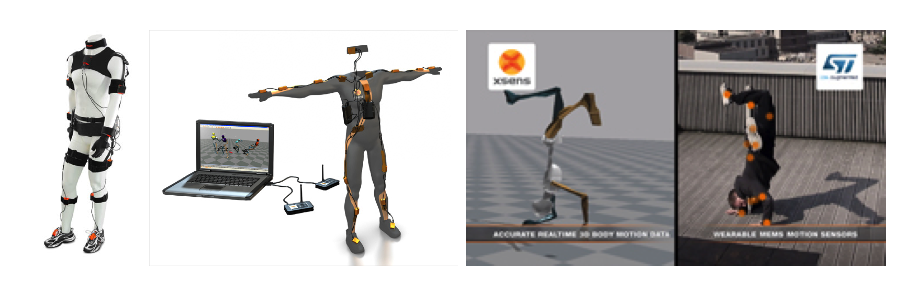
\includegraphics[height=4cm]{images/mvn.png} \includegraphics[height=4cm]{images/mvn2.png} \includegraphics[height=4cm]{images/ST_Xsens.png}
\caption{the images show the commercial product like the Xsens MVN Motion Capture. This system consists of inertial sensors attached to the body by a lycra suit. The motion capture data can be used to animate digital characters in films, games, broadcasted animated stories, ads, serious gaming, virtual environments ea. to get realistic human movement.}\label{fig:xsens}
\end{center}
\end{figure}

In this section we discuss possible industrial applications of the results achieved by the CoDyCo project. A first area of application is definitively an extension of commercial product like the Xsens MVN Motion Capture (see Fig.~\ref{fig:xsens}). This device is a whole-body motion tracking system similar to the well known Vicon system\footnote{\url{http://www.vicon.com}} with some specific advantages like the unlimited tracking volume. This specific device with respect to the Vicon system has the advantage of accessing direct velocity and acceleration measurements which can be used to retrieve full kinematics of each body segment (position, velocity, acceleration, orientation, angular velocity and angular acceleration). Customers of this kind of devices include Sony Pictures Imageworks, Double Negative, Daimler, Electronic Arts, Industrial Light \& Magic, Daimler, INAIL, Ossur and others.


\begin{figure} 
\begin{center}
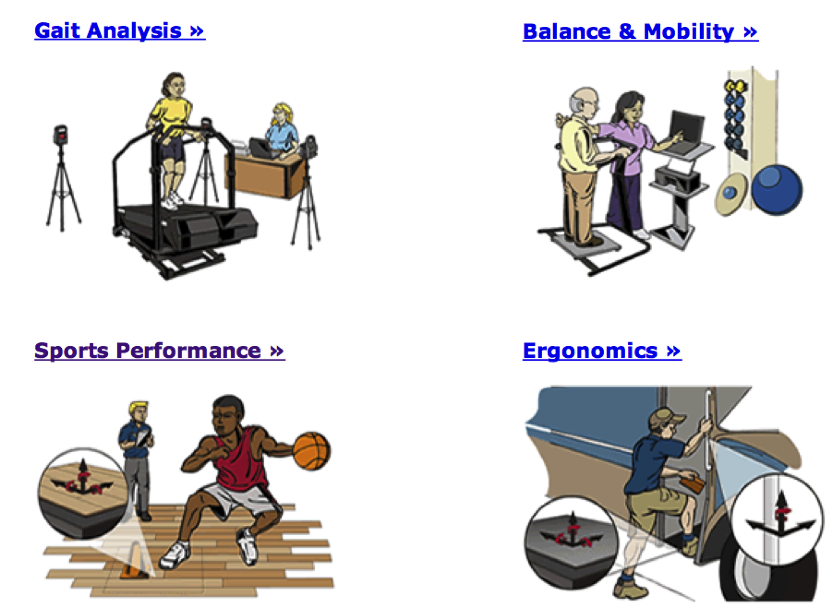
\includegraphics[height=10cm]{images/bertec.png}
\caption{the images show possible applications of devices to measure whole-body interaction forces. This image has been taken from the Bertec company website \protect\url{http://bertec.com}. Bertec is an international industry leader in force measurement technology for biomechanics.}\label{fig:bertec}
\end{center}
\end{figure}

Another possible area of application is the one addressed by the Bertec company, a leading industry in the field of force measurement technology for biomechanics. Fig.~\ref{fig:bertec} show four possible areas of applications ranging from gait analysis, balance mobility, sports performance and ergonomics. Current available technologies are anyway limited to devices to measure the ground reaction forces exchanged between the subject / patient / athlete’s feet and the surface of the platform. 

\begin{figure}
\begin{center}
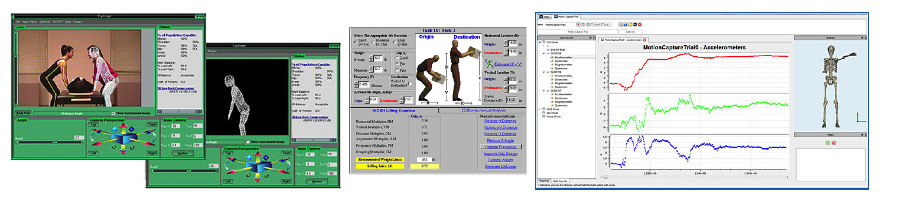
\includegraphics[height=3cm]{images/nexGen.png} \includegraphics[height=3cm]{images/nexGen2.png} \includegraphics[height=3cm]{images/nexGen3.png}
\caption{the images show possible applications in the field of human whole-body motion analysis. This image has been taken from the NexGen Ergonomics company website \protect\url{http://www.nexgenergo.com}. }\label{fig:nexGen}
\end{center}
\end{figure}

NexGen Ergonomics represents another successful company in the field of human whole-body motion analysis. Their activities include: 3D human modeling software, ergonomic design systems, video analysis and other job analysis systems, force measurement systems, EMG analysis systems and data acquisition systems. Here is a list of interesting  NexGen Ergonomics product, pertinent to the CoDyCo scope.
\begin{itemize}
\item The ErgoIntelligence MMH (Manual Material Handling) modules focus on material handling applications and provide an in-depth risk analysis for low-back injury.  This software allows indirect calculation of estimation of energy expenditure. The model can be used to assess whole body fatigue, identify a specific task producing excessive fatigue, or it can be used to determine work-rest ratios. Here is a list of the modules contained in the manual material handling software:
\begin{itemize}
\item EI-MMH-N : NIOSH Lifting Equation with multi-task analysis
\item EI-MMH-NPRO : MMH-N with 2D biomechanics and 2D manikin facility
\item EI-MMH-SCM : Snook \& Ciriello and Mital Table analysis
\item EI-MMH-SCMPRO : MMH-SCM with biomechanics
\item EI-MMH-EE : Energy Expenditure
\end{itemize}
All quantities are indirectly computes and, as such, not specifically tuned on the subject to be analyzed. 

\item The ErgoIntelligence Upper Extremity Assessment (UEA) is a similar tool focused on upper limbs. 

\begin{figure} 
\begin{center}
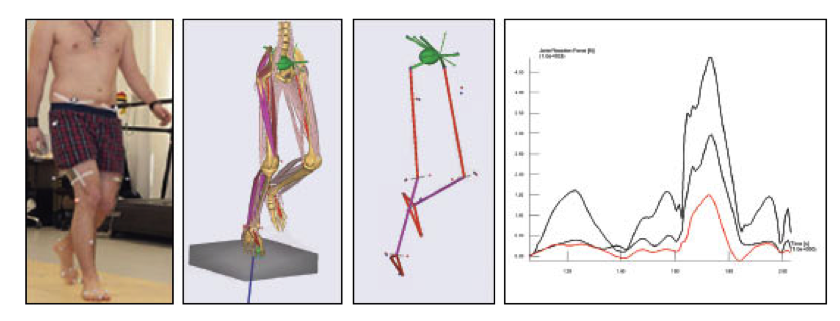
\includegraphics[height=5cm]{images/anyGait.png}
\caption{images of the AnyBody AnyGait software. This is a commercial product of NexGen Ergonomics to obtain sophisticated musculoskeletal analysis of trials. }\label{fig:anyGait}
\end{center}
\end{figure}

\item The AnyBody Modeling System simulates human body movements to estimate individual muscle forces, joint forces and moments, metabolism, elastic energy in tendons and antagonistic muscle actions. Movements are described specifying external forces and posture or motion for the human body (typically acquired with a motion capture system). The AnyBody AnyGait is a tool for gait analysis with the following features: streamlined, intelligent musculoskeletal analysis, easily match the model to each subject, dynamic kinetic and kinematic results. Current analysis uses motion capture data and ground reaction forces. The tool essentially computes inverse dynamics while forward dynamics are still to be implemented.

\end{itemize}




%%\bibliographystyle{alpha}
%%\bibliography{main-bib}

\end{document}

%%% Local Variables:
%%% mode: latex
%%% TeX-master: t
%%% save-place: t
%%% End:
